        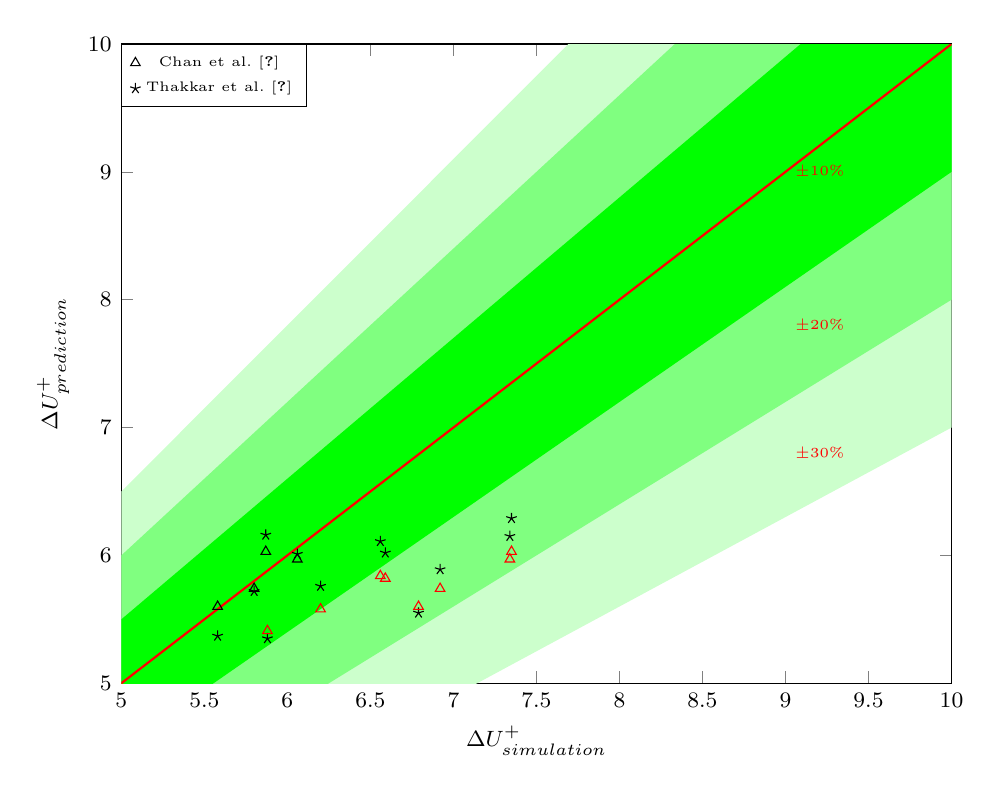
\begin{tikzpicture}[]
        \centering
        \begin{axis}[
            ylabel={$\Delta U_{prediction}^+$},
            xlabel={$\Delta U_{simulation}^+$},
            ymin=5, ymax=10,
			xmax=10,
			xmin=5,
			%xtick={-2,-1.5,...,-0.4},
            width=\linewidth,
            height=.8\linewidth,
            label style={font=\footnotesize},
			legend style={font=\tiny,at={(0,1)},anchor=north west},
            tick label style={font=\footnotesize}
            ]
            \fill[color=green!20,opacity=20] (0,0) -- (10,13) -- (10,7) -- cycle;
            \fill[color=green!50,opacity=50] (0,0) -- (10,12) -- (10,8) -- cycle;
            \fill[color=green!100,opacity=100] (0,0) -- (10,11) -- (10,9) -- cycle;
			\addplot [
            black,only marks,mark=triangle,
            ]
            coordinates{
            (5.87,6.03)
            (6.06,5.97)
            (5.80,5.74)
            (5.58,5.60)
            };
			\addlegendentry{Chan et al.~\cite{chan_macdonald_chung_hutchins_ooi_2015}}
						\addplot [
            black,only marks,mark=star,
            ]
            coordinates{
            (7.35,6.29)
            (7.34,6.15)
            (6.92,5.89)
            (6.79,5.55)
            (6.56,6.11)
            (6.59,6.02)
            (6.20,5.76)
            (5.88,5.35)
            (5.87,6.16)
            (6.06,6.01)
            (5.80,5.72)
            (5.58,5.37)
            };
			\addlegendentry{Thakkar et al.~\cite{Thakkar2017}}
						\addplot [
            red,only marks,mark=triangle,
            ]
            coordinates{
            (6.56, 5.84)
            (6.59, 5.82)
            (6.20,5.58)
            (5.88,5.41)
            (7.35,6.03)
            (7.34,5.97)
            (6.92,5.74)
            (6.79,5.60)
            };
			\addplot [
            red,thick,solid,mark=square,
            ]
            coordinates{
            (0, 0)
            (11, 11)
            };
			\node[red,right] at (axis cs: 9,9) {\tiny $\pm10\%$};
						\node[red,right] at (axis cs: 9,7.8) {\tiny $\pm20\%$};
									\node[red,right] at (axis cs: 9,6.8) {\tiny $\pm30\%$};
        \end{axis}
        \end{tikzpicture}